\label{chap:communication}
\label{sec:communication}

\section{Remote Procedure Calls}
% (Ruda)

We use GWT RPCs.

TODO: describe GWT RPCs

\section{Communication Scheme}
GUI communicates with Userspace via a GWT RemoteService implementation, defined as the FilmTitService interface.
The interface provides asynchronous RPC methods (the responses are processed by callbacks).

The method is always called from the client, because Javascript security policies do not allow to handle incoming calls.
Therefore, in case the Userspace needs to actively contact the GUI without the GUI having sent a request before,
this has to be implemented in the GUI by polling.

\section{Manipulating the documents}

\subsubsection{createDocument}
	Document createDocument(String movieTitle, String year, String language);

Userspace creates a Document instance with the given title, year and language.
It checks the data with IMDB and fills in other information if a corresponding movie is found.
Once the Document is created, it is sent back to the GUI.

\subsubsection{getTranslationResults}
	TranslationResult getTranslationResults(TimedChunk chunk);
	
Userspace passes the given chunk to the core, which generates zero or more translation suggestions.
These are packed into a TranslationResult instance and sent back to GUI.

\begin{figure}[h]
\begin{center}
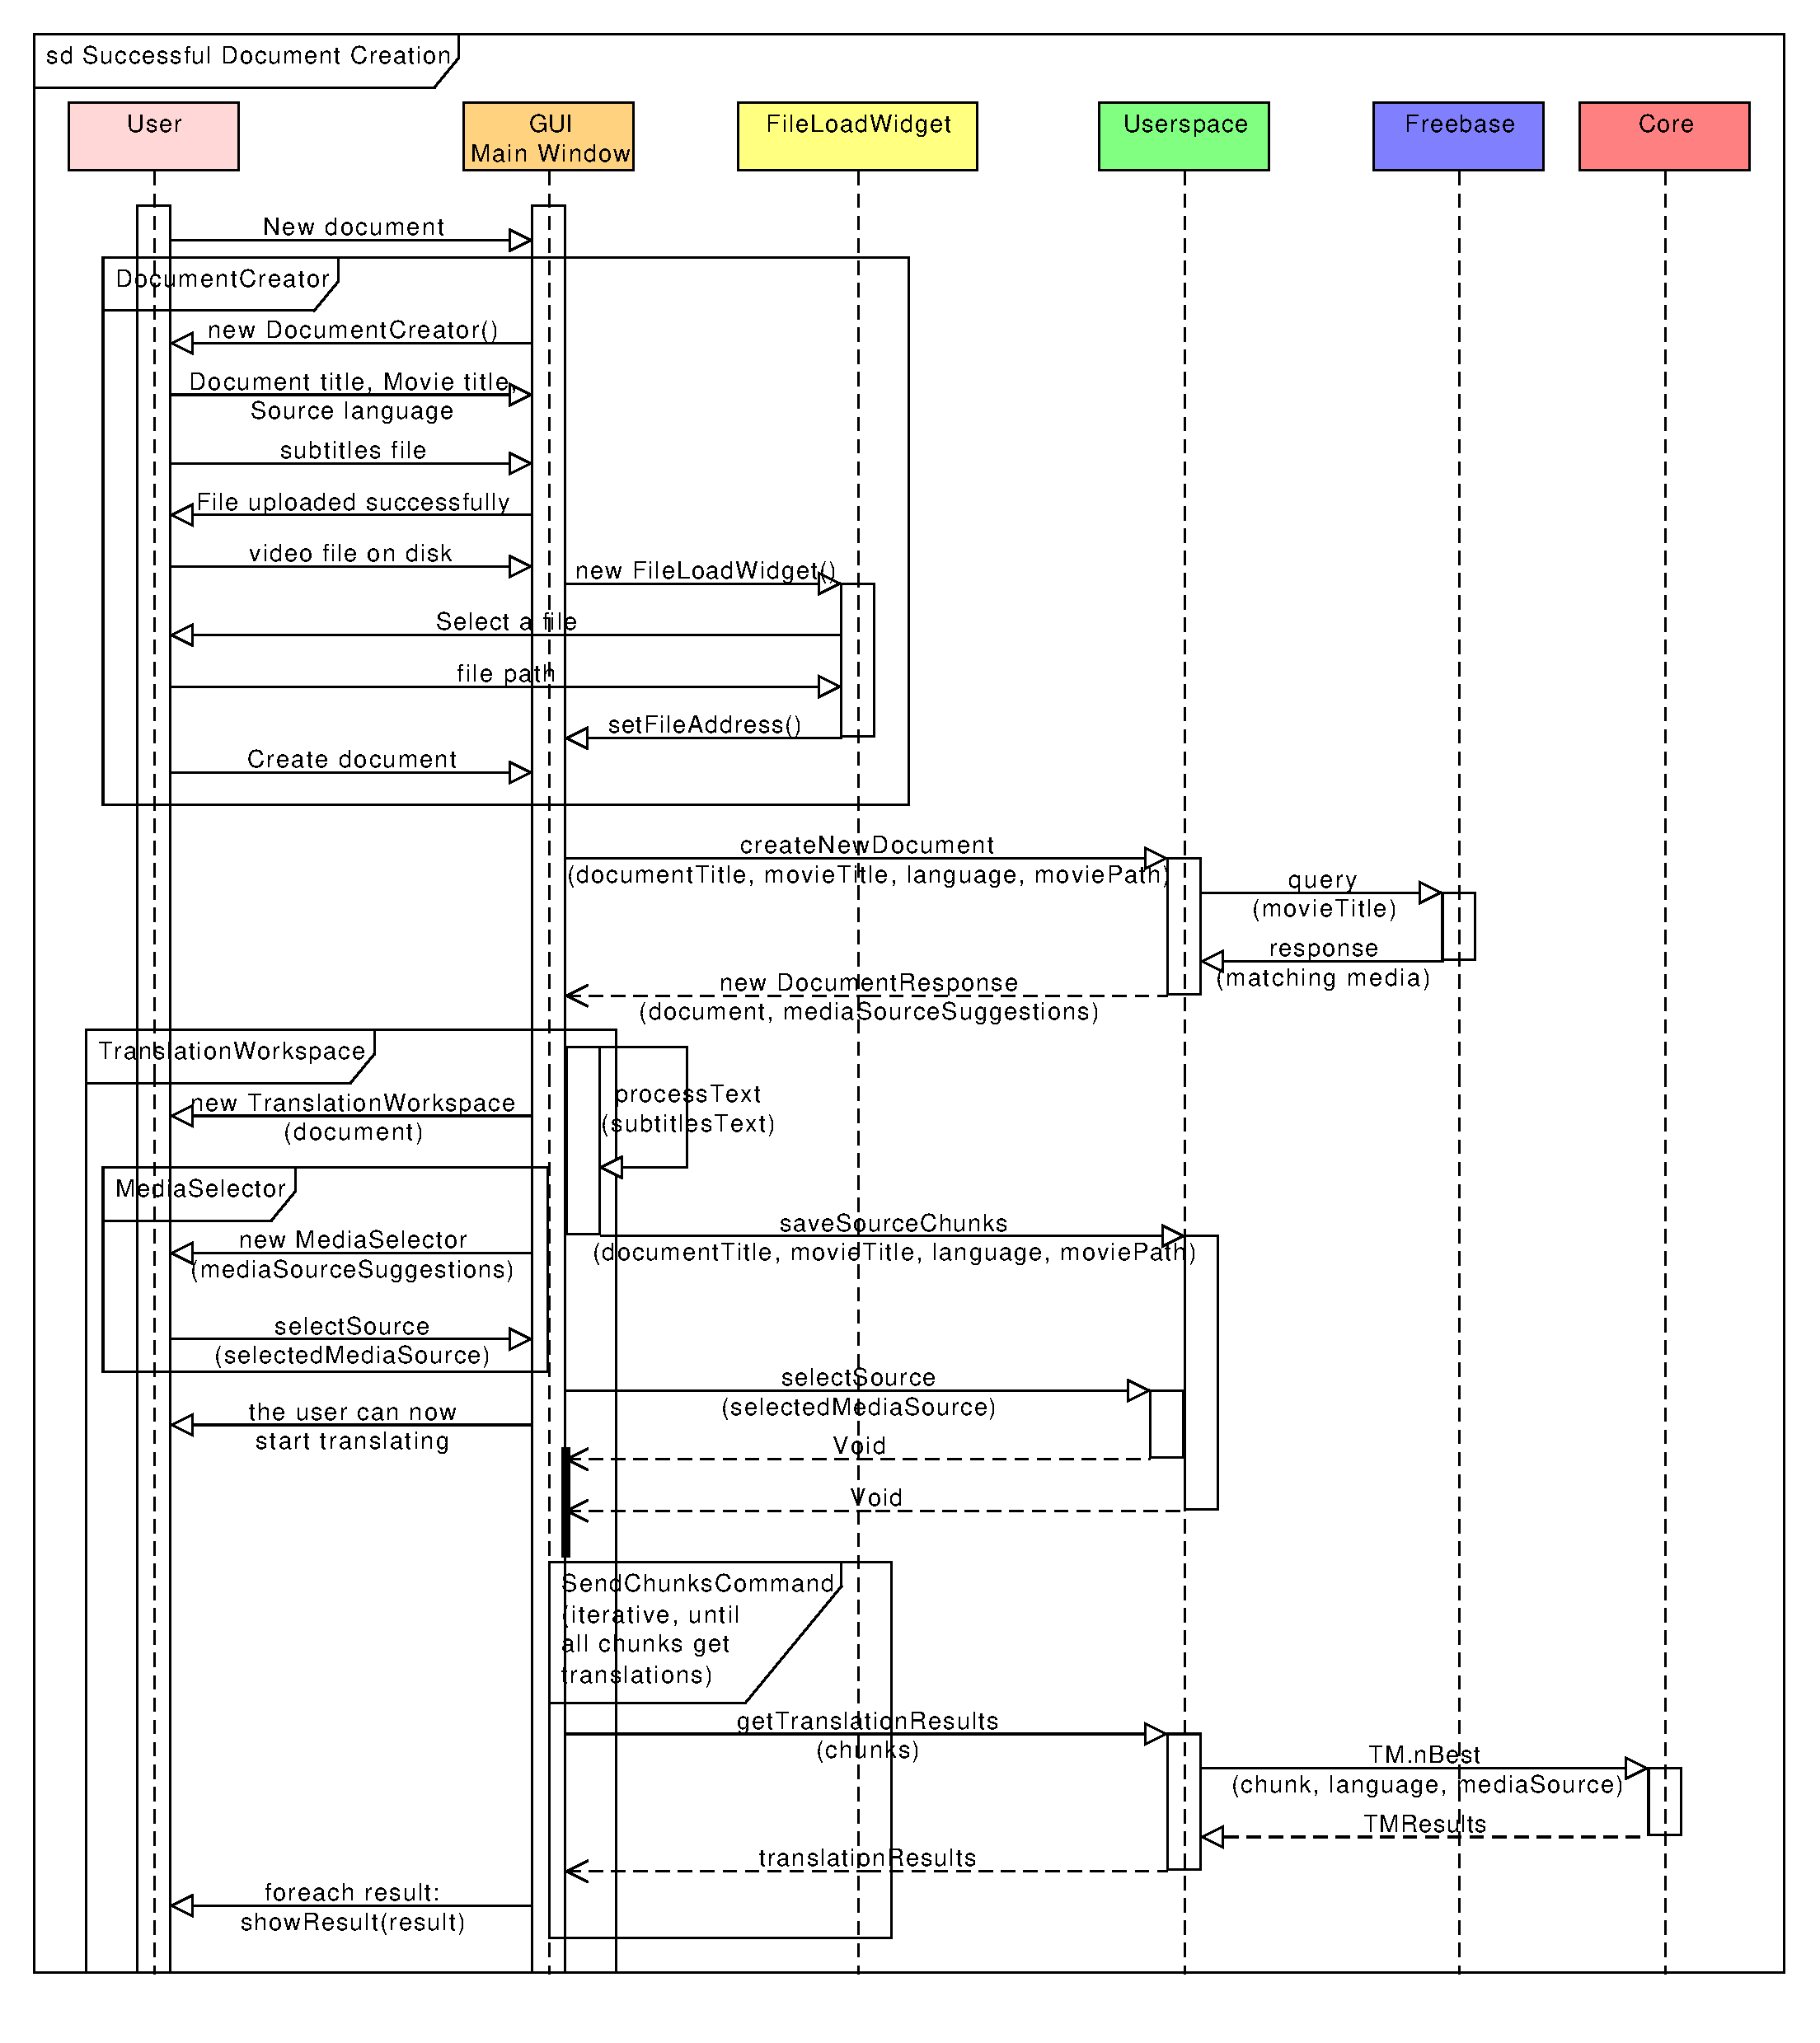
\includegraphics[scale=0.45]{figures/document_creation_sequence.pdf}
\end{center}
\caption{Sequence diagram of document creation, including translation suggestions loading.}\label{gui:sd:document_creation}
\end{figure}

\subsubsection{setUserTranslation}
	Void setUserTranslation(int chunkId, long documentId, String userTranslation, long chosenTranslationPair);

This method is called once the user selects a suggested translation and optionally post-edits it
(or does not select one but inputs the translation text directly).
The translation is then saved by Userspace;
the id of the TranslationPair chosen for post-editing is also sent, providing feedback which then can be used to improve future suggestions.

\section{User login}

The user is required to log in to be able to save his work on the server.
TODO: Do we allow the user to work without being logged in?

The user is logged in if he has a valid session id which is linked to a user account in Userspace.
The session id expires after a given period of time without any user interaction with the server,
it is therefore neccessary that the user can log in without the application\'s main window being reloaded so that the user does not lose unsaved data.

\subsubsection{Simple Login}
\label{subsec:simple_login}

TODO: There is simple login which is very simple. See Figure \ref{gui:sd:simple_login}.


\begin{figure}[h]
\begin{center}
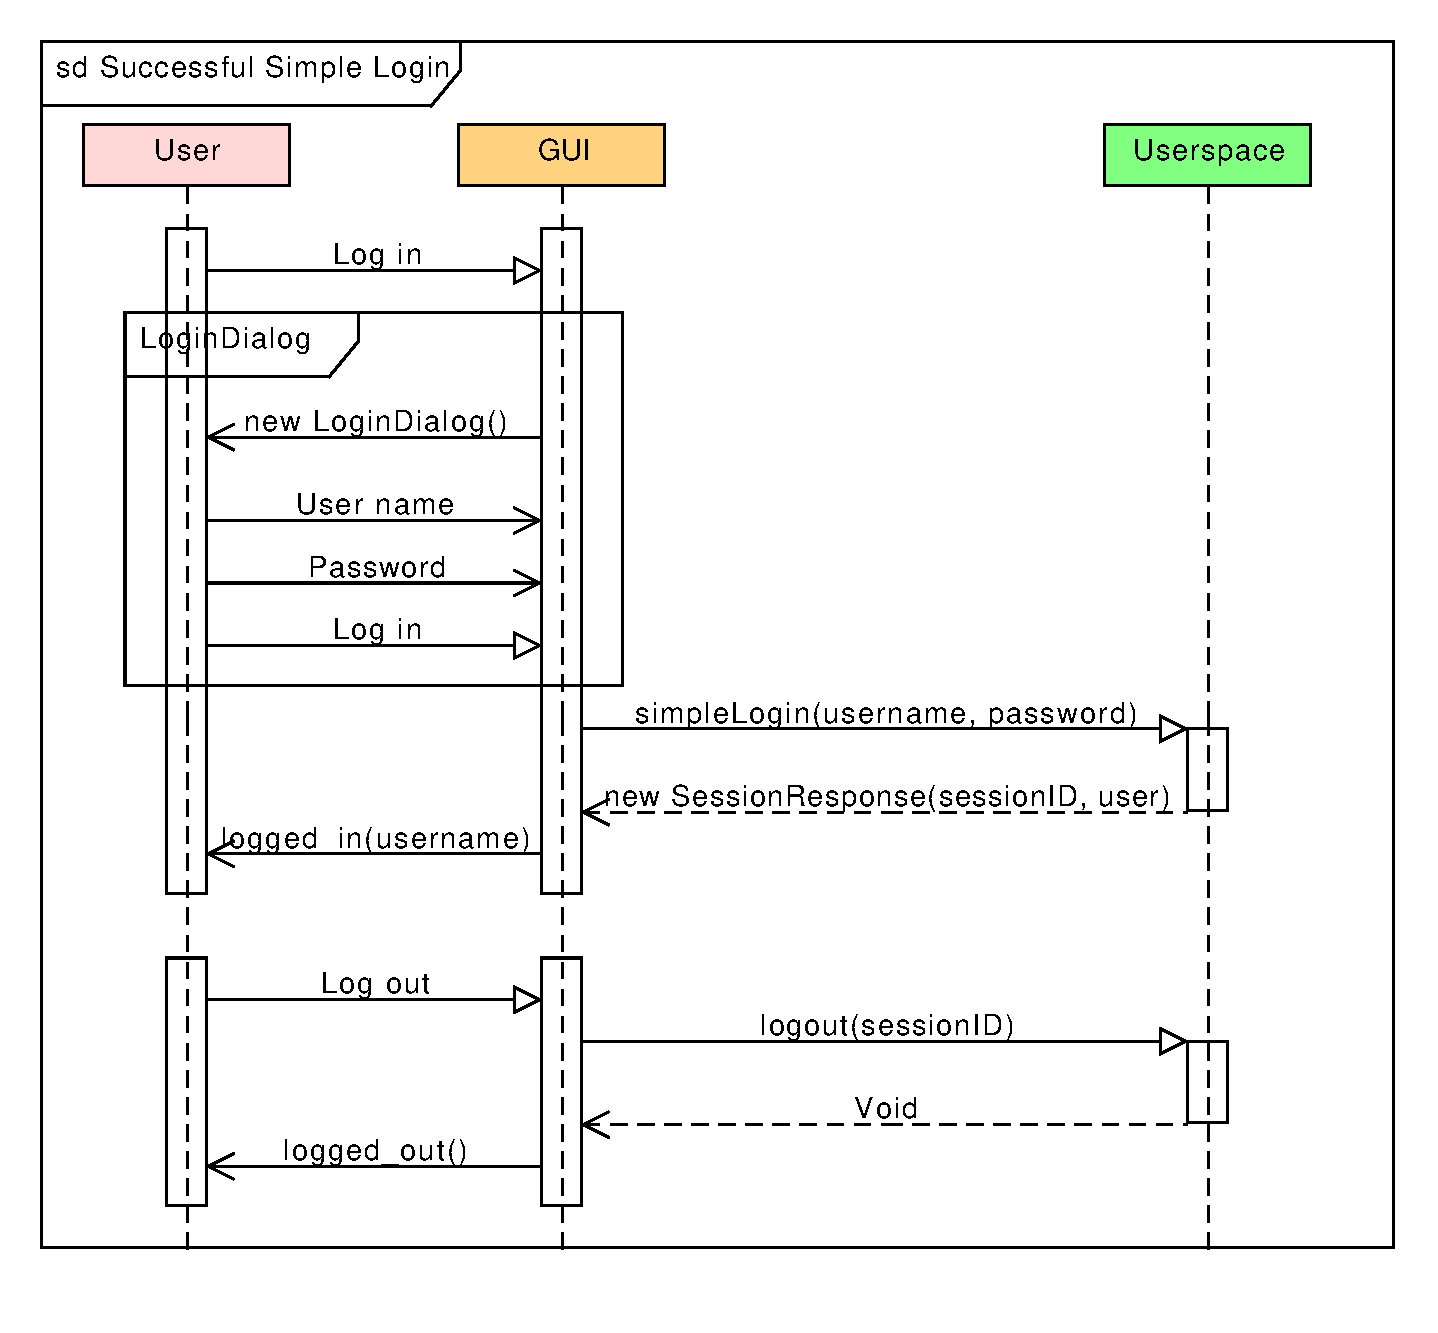
\includegraphics[scale=0.65]{figures/simple_login_sequence.pdf}
\end{center}
\caption{Sequence diagram of simple login and logout.}\label{gui:sd:simple_login}
\end{figure}

\subsubsection{Login via OpenID Services}
\label{subsubsec:gui_openid}

The authentication itself is done in a new authentication window.
A successful authentication is then paired with the GUI instance using a temporary one-time identifier, authID, shared by the main window and the authentication window.
(Because of Javascript security restrictions, there is no simple way of sending the result of the authentication process from the authentication window to the main window;
however, it is straightforward to generate the authID in the main window, store it in Userspace and send it to the authentication window on its creation.)

When the main window requests user authentication, it generates the authID, calls getAuthenticationURL and opens an authentication window with the returned URL.
Then it waits for the user to authenticate in the authentication window
-- the waiting is active, polling the Userspace with getSessionID in regular intervals.
TODO: I suggest every 3 seconds for the first 2 minutes, then every 10 seconds for the following 8 minutes, and then every 30 seconds forever.
And, of course, if the main window regains focus, we call getSessionID immediately.
For each of the authentication services, there is a webpage that enables the user to authenticate
(its URL is returned by getAuthenticationURL)
and then passes information about the result of the authentication to a webpage given to it as a get parameter
(we use the Authentication Response Window as the target webpage).
The result is then sent to Userspace by validateAuthentication.
If the authentication is successful, a new session is created for the user.
The main window then acquires the new session id via getSessionID and the authentication process is completed.

Several ways of authenticating the user are supported, including authentication by Google openID and Facebook account.

\subsubsection{getAuthenticationURL}
    String getAuthenticationURL(long authID, AuthenticationServiceType serviceType);

Called by GUI when authentication is required and the user is not logged in (i.e. does not have a valid sesion id).
A temporary one-time identifier, authID, is generated for the authentification session only to identify the client logging in and sent to Userspace together with the request.
The chosen service to be used for authentication is also given (e.g. Google or Facebook).
The Userspace returns a URL of the webpage to be used for authentication.

\subsubsection{validateAuthentication}
    Boolean validateAuthentication(long authID, String responseURL);

Called from the authentication response window after the user\'s attempt to authenticate themself.
The responseURL contains information from the authentication service to be checked and used by the Userspace.
If the authentication is found to have been successful, a new session is generated for the user and paired with the given authID, and true is returned.
Otherwise, the method returns false.

\subsubsection{getSessionID}
    String getSessionID(long authID);

Userspace checks whether a successful authentication has been done with the given authID.
If yes, the corresponding session id is returned.
Otherwise, null is returned.
TODO null or empty string?
TODO we still need to be able to send info that the user decided to cancel the authentication if we find this out - probably by an exception?

\begin{figure}[h]
\begin{center}
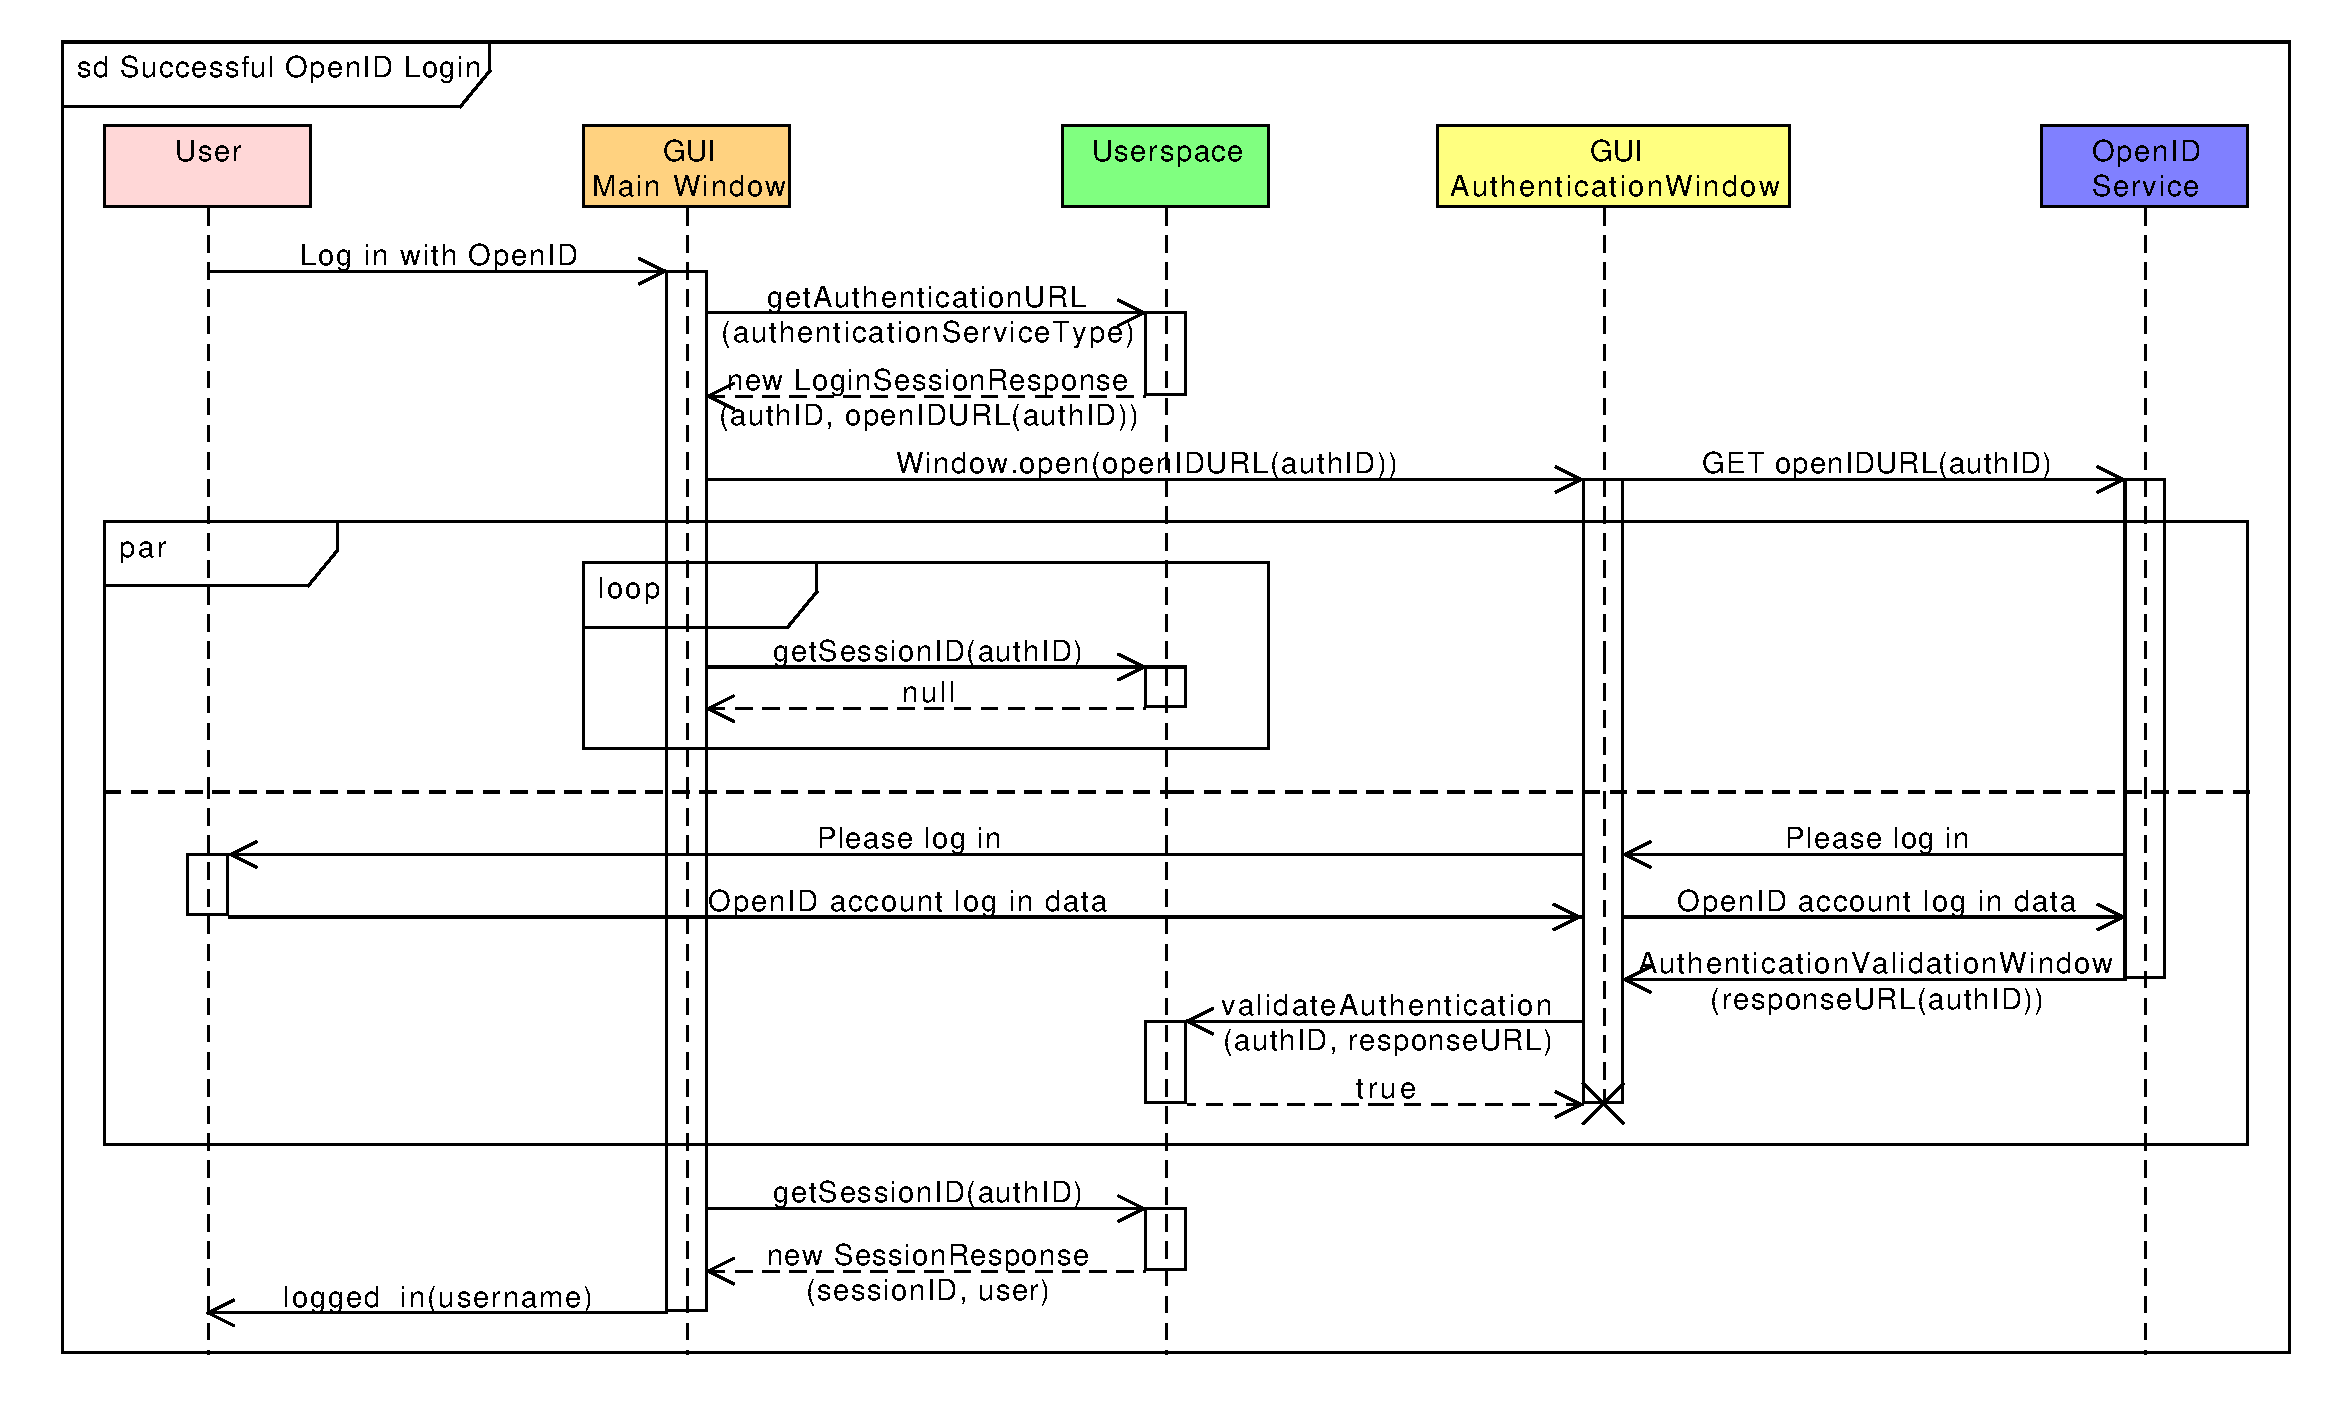
\includegraphics[scale=0.55, angle=90]{figures/openid_login_sequence.pdf}
\end{center}
\caption{Sequence diagram of OpenID login.}\label{gui:sd:openid_login}
\end{figure}
